\documentclass{article}
\usepackage{graphicx}

\title{Popis komponenti za računalo}
\author{Tomislav Magić}
\date{18. siječnja 2024}

\begin{document}
\maketitle
Za računalo namijenjeno CAD programiranju, potrebne su komponente koje pružaju visoke performanse, posebno u području procesiranja i grafičkog prikaza. Ovdje je popis komponenata s nazivima modela koje sam odabrao.

Procesor: Intel Core i7-12700K(12C/20T, 5.0GHz, 25MB, LGA1700) iz 12. generacije. Ovaj procesor nudi visoke performanse s više jezgara i niti, što je važno za CAD programiranje. CAD aplikacije često koriste višestruku nitnu obradu, pa su procesori s visokim brojem jezgara posebno korisni za ubrzanje radnji u CAD okruženju.


Matična ploča: ASUS ROG Strix Z690-E Gaming WiFi(LGA 1700,DDR5,	Intel Z690,128 GB,6400 MHz). Ova matična ploča podržava brzu memoriju, PCIe Gen 4, te ima dodatne funkcije kao što su visokokvalitetni audio i brzu mrežnu vezu. Sve to pridonosi općenitoj stabilnosti i brzini sustava.


RAM memorija: Kingston DDR5 FURY Beast(6000 MHz, 2x16, 32GB, CL40).CAD programiranje može zahtijevati veliku količinu RAM-a, posebno pri radu s velikim projektima ili složenim simulacijama.

Grafička kratica: NVIDIA Quadro RTX 4000(8 GB GDDR6,PCI Express 3.0 x16,1545 MHz, 256 bit).Grafičke kartice iz Quadro serije optimizirane su za rad s CAD aplikacijama. Visoka količina video memorije i certifikacija od strane proizvođača čine ih pouzdanim izborom za CAD programiranje.

SSD: Samsung 970 EVO Plus(M.2, 2TB, 3,500 MB/s).Brzi disk ubrzava učitavanje projekata i smanjuje vrijeme čekanja prilikom otvaranja velikih datoteka u CAD softverima.

Napajanje: RMx Series™ RM750x(750W). Stabilno i pouzdano napajanje ključno je za održavanje radne stabilnosti sustava, posebno pri intenzivnom radu.

Kučište: NZXT H510. Ova kućišta pružaju dobru ventilaciju i olakšavaju održavanje optimalnih radnih temperatura, čime se osigurava dugovječnost komponenti.

Hlađenje: NZXT Kraken X63. Pruža učinkovito hlađenje procesora, čime se osigurava stabilnost sustava tijekom dugotrajnog rada.

Monitor: AOC 24B1H(23,6” FHD, VA Panel, HDMI, D-Sub, AMD FreeSync)
Miš: MS Focus C115
Tipkovnica: MS ELITE C510

Cijene komponenti: procesor - 370€, matična ploća - 321€, RAM - 140€, grafička kratica - 735€, SSD - 165€, napajanje - 160€, kučište - 110€, hlađenje - 154€, monitor - 110€, miš - 6€, tipkovnica - 13€.
Ukupna cijena: 2284€


\begin{figure}
    \centering
    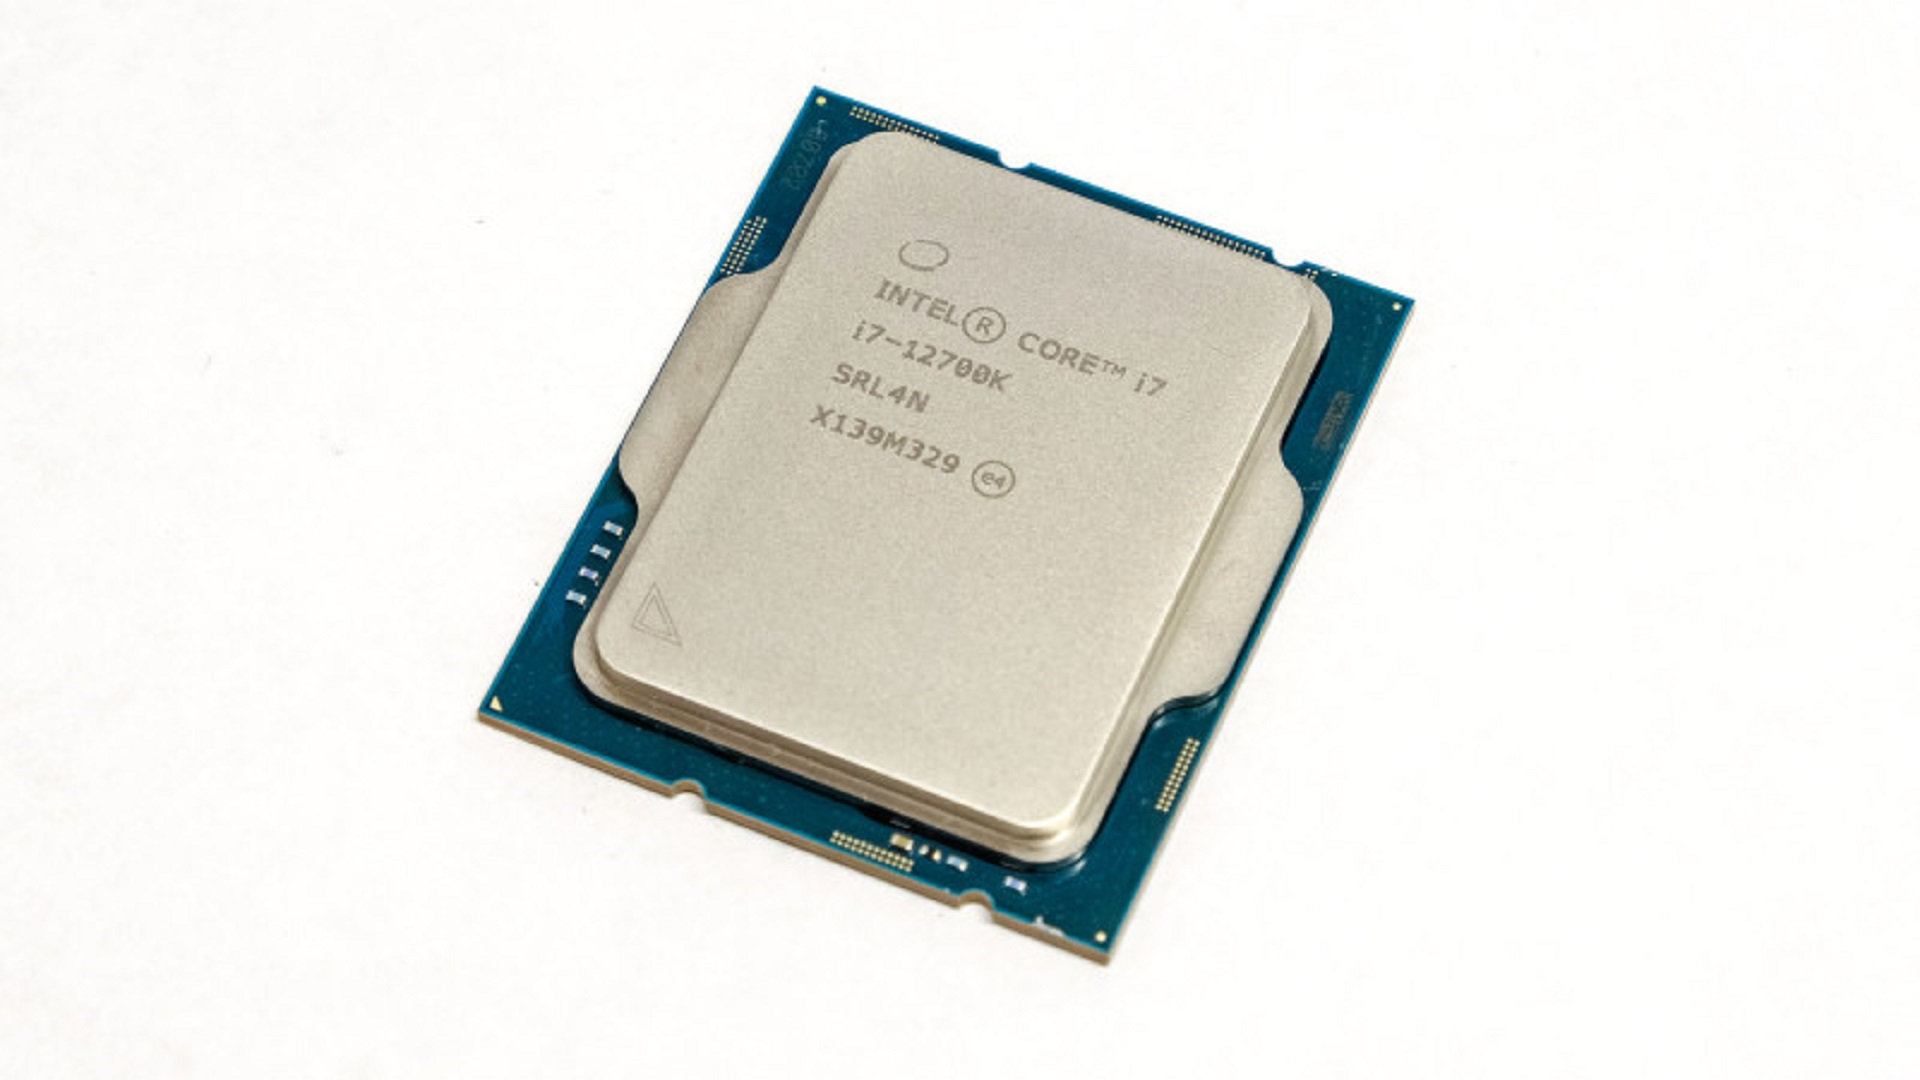
\includegraphics[width=0.5\linewidth]{slike/Intel.jpg}
    \caption{Intel Core i7-12700K}
\end{figure}
\begin{figure}
    \centering
    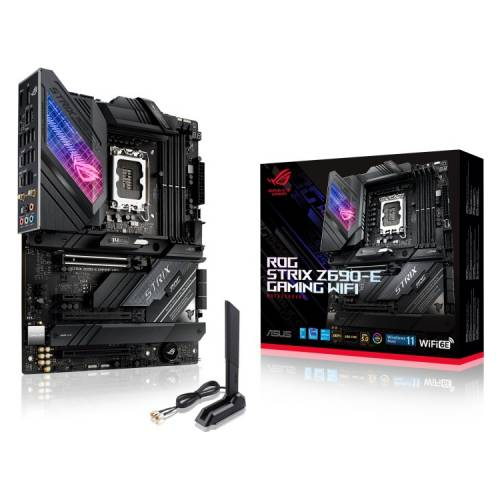
\includegraphics[width=0.5\linewidth]{slike/Asus.jpg}
    \caption{ASUS ROG Strix Z690-E Gaming WiFi}
\end{figure}
\begin{figure}
    \centering
    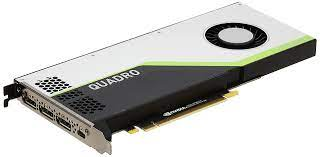
\includegraphics[width=0.5\linewidth]{slike/NVIDIA.jpg}
    \caption{NVIDIA Quadro RTX 4000}
\end{figure}


\end{document}
